% !TEX root = main.tex

%%%%%%%%%%%%%%%%%%%%%%%%%%%%%%%%%%%%%%%%%%%%%%%%%%%%%%%%%%%%
\appendices


\small

\section{Definition of the derivatives in $S3$ and $SO(3)$}
\label{sec:derivatives_SO3}


%%%%%%%%%%%%%%%%%%%%%%%%%%%%%%%%%%%%%%%%%%%%%%%%%%%%%%%%%%%%%
\subsection{Exp and Log maps in $S3$ and $SO(3)$}

We use vectorized versions of the exponential and logarithmic maps in the rotation groups $S3$ (quaternion) and $SO(3)$ (rotation matrix), and denote them with capitalized names $\Exp()$ and $\Log()$ (see \figRef{fig:manifold}, left). They operate directly on the vector space $\bbR^3$, and use either quaternions for $S3$,%as the representation of $SO(3)$,
%
\begin{subequations}
\begin{align}
\bfq
&= \Exp(\bth) \te \begin{bmatrix}
\cos(\theta/2) \\ \bfu\sin(\theta/2)
\end{bmatrix}\\ 
\theta\bfu &= \Log(\bfq) \te 2\,\qv\frac{\arctan({\norm{\qv},q_w})}{\norm{\qv}}
~,
\end{align}
\end{subequations}
%
or rotation matrices for $SO(3)$, 
%
\begin{subequations}
\begin{align}
\bfR
&= \Exp(\bth) \te \bfI + \sin\theta\hatx{\bfu} + (1-\cos\theta)\hatx{\bfu}^2~ \label{equ:rodrigues} \\ 
%\theta &= \cos\inv\left(\frac{\trace(\bfR)-1}{2}\right) \\
\theta\bfu &= \Log(\bfR) \te \frac{\theta(\bfR-\bfR\tr)^\vee}{2\sin\theta} 
~,
\end{align}
\end{subequations}
%
with $\theta=\cos\inv\left(\frac{\trace(\bfR)-1}{2}\right)$,
and where $\bullet^\vee$, known as the \emph{vee} operator, is the inverse of the \emph{skew} operator $\hatx{\bullet}$. 
Their exact form ($\bfq$ or $\bfR$) is always clear by the context.
Since the quaternion implementation is one of our contributions, in the following we will refer to the rotation groups $S3$ and $SO(3)$ with the unique name $S3$, although everything applies equally to $SO(3)$. 

%The equivalence $\bfq\od\bfv=\bfR\bfv$ and the indistinct usage of the $\Exp()$ and $\Log()$ notations allows us to define all the forthcoming IMU-preintegration algebra in a way that allows a direct passage between the $S3$ and $S3$ implementations.
%Therefore, in the following we will refer to the groups $S3$ and $SO(3)$ with the unique name $S3$. 



%%%%%%%%%%%%%%%%%%%%%%%%%%%%%%%%%%%%%%%%%%%%%%%%%%%%%%%%%%%%%
\subsection{The additive and subtractive operators in $S3$ and $SO(3)$}

\begin{figure}[tb]
\begin{center}
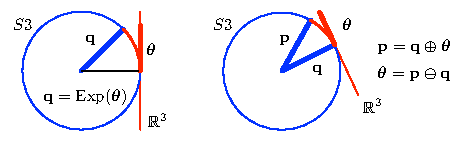
\includegraphics{figures/manifold}
\caption{The S3 manifold is a unit sphere in $\bbR^4$, here represented by a unit circle (blue),  where all unit quaternions live. The tangent space at the element $\bfq$ is the hyperplane $\bbR^3$, here represented by a line (red). The $\Exp()$ and $\Log()$ operators map elements of $\bbR^3$ to/from elements of $S3$. The $\oplus$ and $\ominus$ operators relate elements of the manifold with elements in the tangent space. (Likewise, these figures illustrate the $SO(3)$ manifold.)}
\label{fig:manifold}
\end{center}
\end{figure}




The `plus' operator, $\oplus:S3\times\bbR^3\to S3$, composes a reference element $\sR\in S3$ with a (often small) rotation specified by a vector of $\bth\in\bbR^3$ that is tangent to the $S3$ manifold at $\sR$, yielding an element $\sS\in S3$ (see \figRef{fig:manifold}, right). 
%
%\begin{align*}
%\sS = \sR\oplus \bth &\te \sR\circ\Exp(\bth) && \sR,\sS\in S3,~ \bth\in\bbR^3 
%\end{align*}
%
The `minus' operator, $\ominus:S3\times S3\to\bbR^3$ is the inverse of the above.
%
%\begin{align*}
%\bth=\sS\ominus \sR
%&\te \Log(\sR\inv \circ \sS)     && \sR,\sS\in S3,~ \bth\in\bbR^3  
%\end{align*}
%
These operators are defined for both $\bfq$ and $\bfR$,
%
\begin{align}
\bfq\oplus\bth  &= \bfq\ot\Exp(\bth) \\
\bfR\oplus \bth &= \bfR\Exp(\bth) \\
\bth = \bfp\ominus\bfq &= \Log(\bfq^*\ot\bfp) \\
\bth = \bfS\ominus\bfR &= \Log(\bfR\tr\,\bfS)                         
\end{align}


%%%%%%%%%%%%%%%%%%%%%%%%%%%%%%%%%%%%%%%%%%%%%%%%%%%%%%%%%%%%%
\subsection{The four possible derivative definitions}

For functions $f:\bbR^m\to\bbR^n$, we use the standard operators $\{+,-\}$ to define the derivative as
%
\begin{align}
\dpar{f(\bfx)}{\bfx} &\te \lim_{\delta\bfx\to0}\frac{f(\bfx+\delta\bfx)-f(\bfx)}{\delta\bfx} &&\in \bbR^{n\times m} \label{equ:derivative_vector}
\end{align}
%
For functions $g:S3\to S3$, we use the operators $\{\oplus,\ominus\}$,
%
\begin{align}
\dpar{g(\sR)}{\bth} 
&\te \lim_{\delta\bth\to0}\frac{g(\sR\oplus\delta\bth)\ominus g(\sR)}{\delta\bth}  && \in \bbR^{3\times 3}
\label{equ:derivative_SO3}
\end{align}
%
For functions $h:\bbR^m \to S3$, we use $\{+,\ominus\}$,
%
\begin{align}
\dpar{h(\bfx)}{\bfx} &\te \lim_{\delta\bfx\to0} \frac{ h(\bfx+\delta\bfx)\ominus h(\bfx)}{\delta\bfx} && \in \bbR^{3\times m} \label{equ:dif_RtoSO3}
\end{align}
%
For functions $k:S3\to\bbR^n$, we use $\{\oplus,-\}$,
%
\begin{align}
\dpar{k(\sR)}{\bth} &\te \lim_{\delta\bth\to0} \frac{k(\sR\oplus\delta\bth) - k(\sR)}{\delta\bth} && \in \bbR^{n\times 3} \label{equ:jacobian_SO3_Rn}
\end{align}


%%%%%%%%%%%%%%%%%%%%%%%%%%%%%%%%%%%%%%%%%%%%%%%%%%%%%%%%%%%%%
\subsection{Right Jacobian of $S3$ and $SO(3)$}

We define the right Jacobian as, 
%
\begin{align}\label{equ:Jr}
\bfJ_r(\bth) &\te \dpar{\Exp(\bth)}{\bth} 
\in\bbR^{3\tcross3}
\end{align}
%
We implement this derivative using \eqRef{equ:dif_RtoSO3}.
The right Jacobian can be computed in closed form  \cite[pag.~40]{CHIRIKJIAN-12} with
%
\begin{align}
\bfJ_r(\bth) &= \bfI - \frac{1-\cos\nth}{\nth^2}\hatx{\bth} + \frac{\nth-\sin\nth}{\nth^3}\hatx{\bth}^2 
\end{align}



%%%%%%%%%%%%%%%%%%%%%%%%%%%%%%%%%%%%%%%%%%%%%%%%%%%%%%%%%%%%%
\subsection{Examples}

\subsubsection{Function $\bbR^3\to S3$} 
\label{sec:jac_R3toSO3}

The function $f(\bw) = \Exp(\bw\dt)$ produces elements of $S3$ from vectors $\bw\in\bbR^3$. 
Its Jacobian \wrt $\bw$ follows from \eqRef{equ:dif_RtoSO3}, but is better obtained from \eqRef{equ:Jr} and the chain rule,
%
\begin{align*}
\dpar{\Exp(\bw\dt)}{\bw}
= \dpar{\Exp(\bw\dt)}{(\bw\dt)}\dpar{(\bw\dt)}{\bw} 
= \bfJ_r(\bw\dt)\dt
\end{align*}
%


\subsubsection{Function $S3\times\bbR^3\to\bbR^3$} 
\label{sec:jac_SO3xR3toR3}

The rotation $f(\sR,\bfv) = \bfq\od\bfv = \bfR\,\bfv$ produces vectors of $\bbR^3$ from elements $\sR\in S3$ and vectors $\bfv\in\bbR^3$. The first Jacobian is defined by \eqRef{equ:jacobian_SO3_Rn} and developed as
%
\begin{align*}
\dpar{\bfq\od\bfv}{\bth} = \dpar{\bfR\bfv}{\bth} 
&\te \lim_{\delta\bth\to0}\frac{(\bfR\oplus\delta\bth)\bfv-\bfR\bfv}{\delta\bth} \\
= \lim_{\delta\bth\to0}\frac{\bfR\Exp(\delta\bth)\bfv-\bfR\bfv}{\delta\bth} 
&= \lim_{\delta\bth\to0}\frac{\bfR\tdot(\bfI+\hatx{\delta\bth})\bfv-\bfR\bfv}{\delta\bth} \\
= \lim_{\delta\bth\to0}\frac{\bfR\hatx{\delta\bth}\bfv}{\delta\bth} 
&= \lim_{\delta\bth\to0}\frac{-\bfR\hatx{\bfv}\delta\bth}{\delta\bth} 
= -\bfR\hatx{\bfv} 
\end{align*}
%
where we used the properties $\Exp(\dth) \approx \bfI + \hatx{\dth}$ and  $\hatx{\bfa}\bfb = -\hatx{\bfb}\bfa$. 
The second Jacobian is defined by \eqRef{equ:derivative_vector} and yields,
%
\begin{align*}
\dpar{\bfq\od\bfv}{\bfv} = \dpar{\bfR\bfv}{\bfv} 
&\te \lim_{\partial\bfv\to0}\frac{\bfR\tdot(\bfv+\partial\bfv)-\bfR\bfv}{\partial\bfv} 
= \bfR
~.
\end{align*}





